\documentclass[10pt]{article}

\title{Characterizing tandem fin wake interaction using lateral line inspired sensors}
\author{MIDN 2/C Cameron Smith\thanks{Department of Weapons, Robotics, and Control Engineering at the United States Naval Academy. Address for correspondence \emph{m226072@usna.edu}}}
\date{\today}
\usepackage[separate-uncertainty=true]{siunitx}
\usepackage{amsmath,amsfonts,amssymb}
%\DeclareSIUnit{\sec}{s}
%\DeclareSIUnit{\centimeter}{cm}
%\DeclareSIUnit{\meter}{m}
%\DeclareSIUnit{\kilogram}{kg}
\usepackage[plain]{fancyref}
\usepackage{listings}
\usepackage[utf8]{inputenc}
\usepackage{booktabs}
\usepackage{graphicx}
\usepackage[round,authoryear]{natbib}
\bibliographystyle{apalike}
\begin{document}
\maketitle
\begin{abstract}

    Fish have demonstrated extreme agility underwater, a desirable trait for unmanned underwater vehicles (UUVs). Much of a fish's maneuverability can be attributed to the complex interactions between the wakes made by its multiple control surfaces. One such interaction of great interest to this project is the interference between vortex wakes produced by the dorsal and caudal fins. The degree of thrust increase from these interactions is influenced by the phase difference between the flapping fins. To incorporate this type of movement in bio-inspired vehicles, it is desirable to develop a feedback architecture that detects the degree of wake interaction.
    %This research project will work toward the development of a feedback control loop for two, two-dimensional tandem fins. In previous work, pressure sensor arrays have accurately characterized single vortex streets. This project will study their response to double vortex wakes to develop a system that provides real-time feedback on tandem foil wake interactions. The pressure sensor array for this project is inspired by the lateral line in fish, an organ that detects flow oscillations.
    
    The goal of this project is to engineer a two dimensional tandem fin system capable of coordinating flapping foils to improve thrust generation using an array of pressure sensors inspired by the fish lateral line system. This research draws inspiration from the flow control properties of dorsal and caudal fin coordination in bony fish and their ability to sense important fluid properties with their lateral line. It also applies observations and techniques used by previous teams to study single vortex wakes using artificial lateral lines. Several experimental trials will be performed in USNA's Large Re-Circulating Water Tunnel to collect wake pressure data downstream from two tandem fins flapping at multiple phase differences. Based on these trials, features of the data will be found that vary according to phase difference. Relationships between these features and the known phase difference will be found using nonlinear methods, enabling a system to map observed wake features to upstream phase difference.
    
    Progress in this field will be beneficial, as control systems capable of calculating tandem foil phase difference will directly relate it to foil thrust production. This will enable more robust and agile underwater locomotion, which contributes to the ability to perform dexterous tasks in difficult environments, such as closely studying coral reefs, maneuvering through subsea obstacles, and UUV schooling.
    
\end{abstract}
% anatomy wise - dorsal fin on a whale is at 90 deg to the 
% tail flukes.. previous usna work dealt with humpback whale
% pectoral fin which does not have an upstream thing 
{\scriptsize Keywords: flapping foil, sensing, biomechanics, hydrodynamics, maneuvering, lateral line, tandem foils}
\tableofcontents
\clearpage
\section{Natural Systems} \label{Natural Systems}

    To create a bio-inspired control system for underwater locomotion, it is necessary to understand the basic morphology of fish and the physical properties of the water they manipulate to achieve their impressive agility. After understanding the structures and behaviors observed in  nature, they can be replicated in laboratory environments and applied to human designs. Drawing inspiration from a fish's mode of underwater sensing will present a method for closing the control loop in fish-inspired propulsion.

\subsection{Karman Vortex Streets} \label{Karman Vortex Streets}

    When fluids flow past bluff bodies, the bodies undergo a periodic cycle of forming and shedding low pressure regions on their downstream sides as the fluid imparts a drag force. These pressure regions consist of swirling fluid and are known as vortices. Each vortex circulates in the opposite direction of the previously shed vortex, and the wake of the bluff body becomes a line of oppositely rotating vortices shed from opposite sides of the body. This phenomenon was often observed, but it was little understood or studied before the publications from Theodore von Karman in 1911 \citep{Karman1911}. As such, the classic vortex wake formed by a smooth cylinder, shown in \Fref{fig:app:Karman}, is known as a Karman vortex street. For a bluff body, the vortex shedding frequency is related to a dimensionless parameter known as the Strouhal number 
    \begin{equation} \label{Eq:Karman St}
    St=\frac{fD}{U_\infty}
    \end{equation} 
    where \(f\) is the vortex shedding frequency, \(U_\infty\) is the free stream velocity, and \(D\) is the characteristic length of the body. In the case of a cylinder, \(D\) is the diameter. As the vortices rotate, the water between them forms jets with less momentum in the flow direction than the water upstream of the bluff body, which indicates a force imposed on the fluid by the body. In general, the force applied on a mass of water at two points in time is related by \[\int_{t_1}^{t_2} \vec F \, dt=m(\vec v_2-\vec v_1)\] where \(\vec F\) is the average force, \(t_1\) and \(t_2\) are the times at two moments, \(m\) is the mass of the water, and \(\vec v_1\) and \(\vec v_2\) are the fluid velocities at the two moments. By Newton's Third Law, the force applied on the water by a bluff body to create vortices is also applied on the bluff body by the water. The vortices, therefore, are a product of the force interaction between a bluff body and the surrounding fluid, and their characteristics vary based on the drag force imposed on the body.

\begin{figure}
\begin{center}
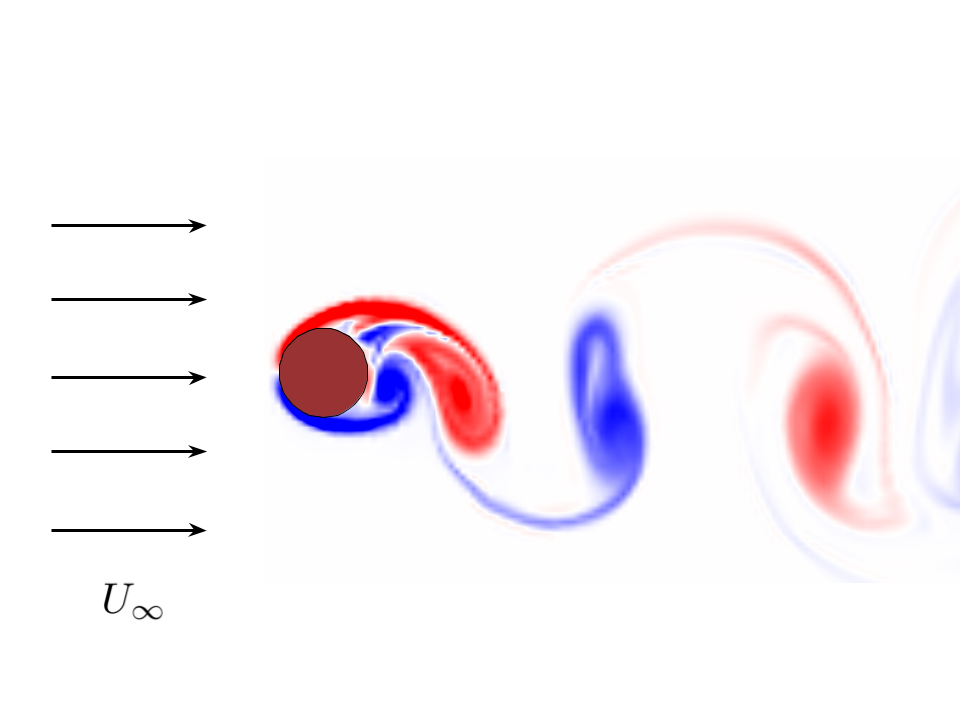
\includegraphics[width=0.6\columnwidth]{figures/Edited Karman Street.png}
\end{center}
\caption{Karman vortex street formed behind a circular cylinder in uniform flow, simulated in Lily Pad computational fluid dynamic (CFD) software \citep{Weymouth2015}. Arrows indicate the direction of free stream fluid flow, $U_\infty$. Red regions indicate clockwise flow, whereas blue regions indicate counterclockwise flow. Color intensity corresponds directly to the circulation intensity, also known as vorticity.}
\label{fig:app:Karman}
\end{figure}

\subsection{Fin Propulsion} \label{Fin Propulsion}

	 Beneath the surface of the water, organisms must contend with higher viscosity, larger drag forces, and often more prevalent predation than organisms that move through air. To overcome these challenges, marine animals, such as cartilaginous and bony fish, have developed the ability to use multiple control surfaces in tandem, enabling smaller turn radii and increased efficiency \citep{Bandyopadhyay2002,Lauder2004,Triant2020,Drucker2001}, which indicates improved agility. \Fref{fig:app:Bluegill} shows the basic fin placement of a ray finned fish using the well studied bluegill sunfish. \citep{Drucker2001} and \citep{Akhtar2007} observed that during forward propulsion ray finned fishes beat the water with their dorsal fins and caudal fins in a periodic motion consisting of two steps: heave and pitch. As \Fref{fig:app:Bluegill} illustrates, the pitch motion is the angular change in the fin’s orientation, while the heave motion is its lateral translation. The movement of a single fin is of the form 
\begin{equation} \label{Eq:Single foil heave}
Heave:  y(t)=Asin(2\pi f_h t)
\end{equation}
\begin{equation} \label{Eq:Single foil pitch}
Pitch: \theta (t)=\theta _msin(2\pi f_h t+\psi)
\end{equation}
    where \(y(t)\) is the position of the fin's leading edge, \(A\) is its amplitude, \(f_h\) is the flapping frequency in Hz, \(\theta(t)\) is the orientation of the fin relative to an inertial reference frame aligned with the incoming uniform flow, \(\theta _m\) is the maximum pitch, \(\psi\) is the phase shift between the two components of the fin motion, and \(t\) is the instantaneous time. During forward movement, the fins create vortex wakes that are nearly identical to those described in Section \ref{Karman Vortex Streets}, except the signs of the vortices are flipped. This street is known as a reverse Karman vortex street. The water momentum jet imposed by a standard Karman vortex street has less velocity in the flow direction, but in the reverse street, the velocity is higher. This is indicative of a thrust force, rather than a drag force. The Strouhal number describing this behavior becomes
    \begin{equation}\label{Eq:Fin St}
        St=\frac{2Af_h}{U_\infty}
    \end{equation}
    where the characteristic length, \(2A\), is the peak to peak amplitude of the oscillating fin. As generalized by \citep{Triant1993}, this  value ranges from 0.2-0.4 for nearly all animals that flap foils for propulsion, including insects, birds, bats, and fish, and this range is associated with the optimized energy input and thrust output. In the case of most bony fish, this value is near 0.25 for steady, forward propulsion \citep{Drucker2001, Nudds2014}.
    
\begin{figure}
\begin{center}
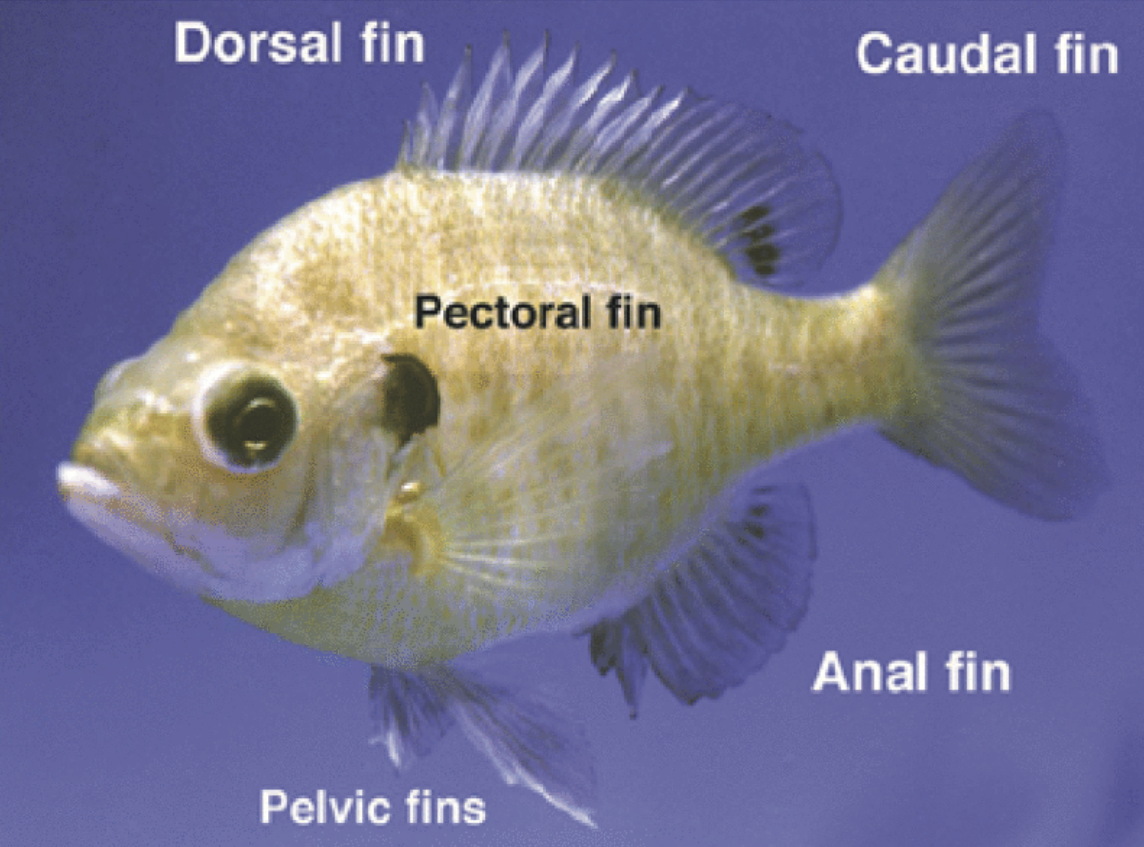
\includegraphics[width=0.44\columnwidth]{figures/Figure1.png}
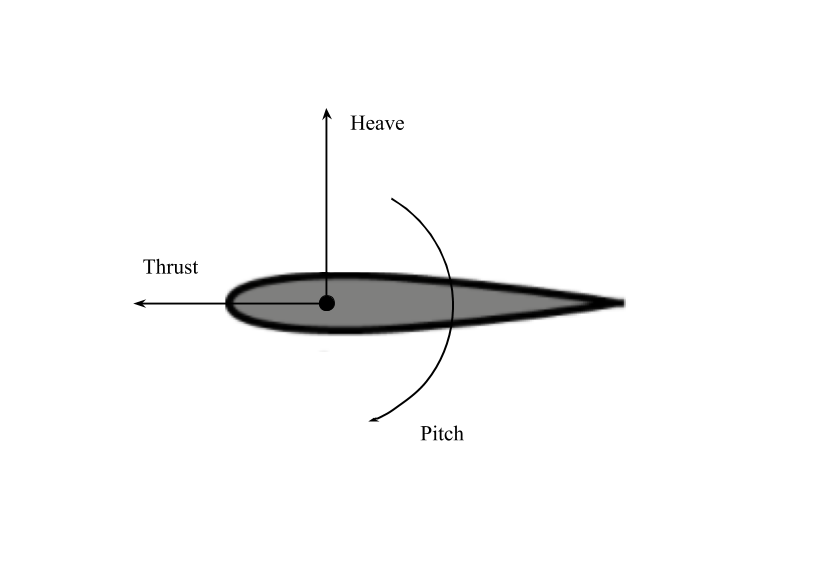
\includegraphics[width=0.54\columnwidth]{figures/Fin Frame.png}
\end{center}
\caption{Diagram of the fin arrangement on bluegill sunfish (left) \citep{Lauder2004}. Top-down view of a fin cross section with a superimposed coordinate grid (right).}
\label{fig:app:Bluegill}
\end{figure}

    During forward movement, the vortex street induced by the dorsal fin flows over the caudal fin, interfering with the caudal fin’s vortices \citep{Drucker2001, Akhtar2007}. This practice allows fish to change the effective angle of attack on their caudal fin and generate improved thrust, power, and efficiency. To reach these goals, the fins flap out of phase with one another \citep{Drucker2001}, and the phase difference causes the effective coefficient of thrust on the caudal fin to change, as shown in \Fref{fig:app:Fish Thrust}. This thrust coefficient, \(C_f\) is related to the fin's instantaneous thrust force by \[C_f=\frac{F}{0.5\rho U_\infty^2 A}\] where \(F\) is the thrust force, \(\rho\) is the water density, \(U_\infty\) is the free stream water velocity, and \(A\) is the fin surface area exposed to the flow. The dorsal fin moves according to (\ref{Eq:Single foil heave}) and (\ref{Eq:Single foil pitch}), while the caudal fin moves according to
    \begin{equation}
Heave: y_c(t)=A_csin(2\pi f_h t+\phi)
\end{equation}
\begin{equation} \label{Eq:Caudal fin pitch}
Pitch: \theta_c (t)=\theta _{mc}sin(2\pi f_h t+\psi+\phi)
\end{equation}
    where \(\phi\) represents the phase difference between the two fins, \(A_c\) represents the caudal fin's heave amplitude, and \(\theta_{mc}\) represents its maximum pitch angle. For bluegill sunfish and other ray finned fishes, \(A_c\) and \(\theta_{mc}\) are slightly greater than their dorsal counterparts \citep{Drucker2001}, although specific values vary depending on the fish species and behavior observed. The optimal \(\phi\) for a pair of tandem fins differs depending on anatomy and fin spacing. For the frequently studied bluegill sunfish shown in \Fref{fig:app:Bluegill}, maximum thrust is achieved at a phase difference of $\phi=48^o$, while other phase differences can achieve smaller increases or even decreases in thrust \citep{Akhtar2007}.

\begin{figure}
\begin{center}
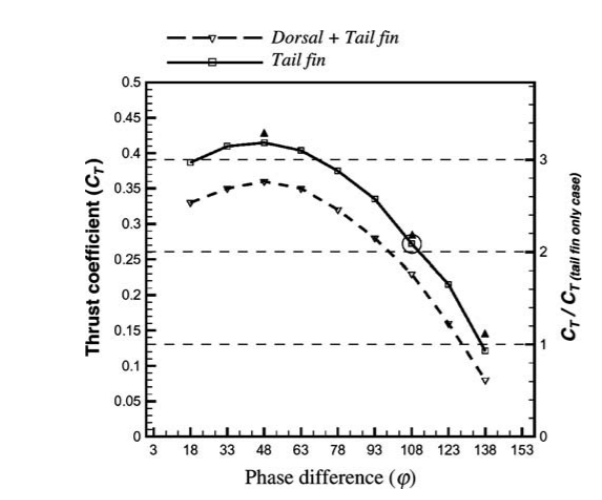
\includegraphics[width=0.49\columnwidth]{figures/Figure2.png}
\end{center}
\caption{Variation of caudal fin thrust coefficient with phase difference. The vertical axis is the thrust coefficient in absolute and normalized terms, while the phase difference is in degrees \citep{Akhtar2007}.}
\label{fig:app:Fish Thrust}
\end{figure}

\subsection{The Lateral Line Organ} \label{The Lateral Line Organ}

	Fish possess a unique sensory organ that allows them to detect both smooth and oscillating flow over their bodies: the lateral line. The line consists of a network of superficial and canal-embedded neuromasts, which deflect when fluid flows past them and stretch clusters of hair cells. These hair cells, in turn, trigger neurons to fire and transmit signals to the fish’s brain \citep{Dijkgraaf1962}. The general layout of the lateral line and the basic structure of the neuromasts are depicted in \Fref{fig:app:Lat Line}. The superficial neuromasts (SN) exist on the fish’s skin and protrude into the boundary layer. These sensors detect slow, steady changes in flow and have been characterized as velocity-sensitive \citep{Montgomery2001}. They typically detect flow changes that take place below 30 Hz \citep{Coombs2001}. The second group, the canal neuromasts (CN), exist as domed structures within small, fluid-filled canals that run beneath the surface of the fish’s skin. This canal is exposed to the outside flow through a series of pores. A CN perceives oscillating flow as pressure differences; when the pressure at one pore is different from the pressure at a pore farther down the canal, the canal fluid moves toward the pore of lower pressure, causing a deflection in the CN. When pressure changes slowly, typically below 30 Hz, the viscous forces within the canals prevent fluid movement \citep{Denton1989}, effectively acting as a high pass filter for pressure frequencies. Thus, CNs typically sense changes in flow that take place between 30 Hz and 150 Hz \citep{Coombs2001}. The pressure difference perceived by CNs can also be interpreted as a flow acceleration across the surface of the fish.
	
\begin{figure}
\begin{center}
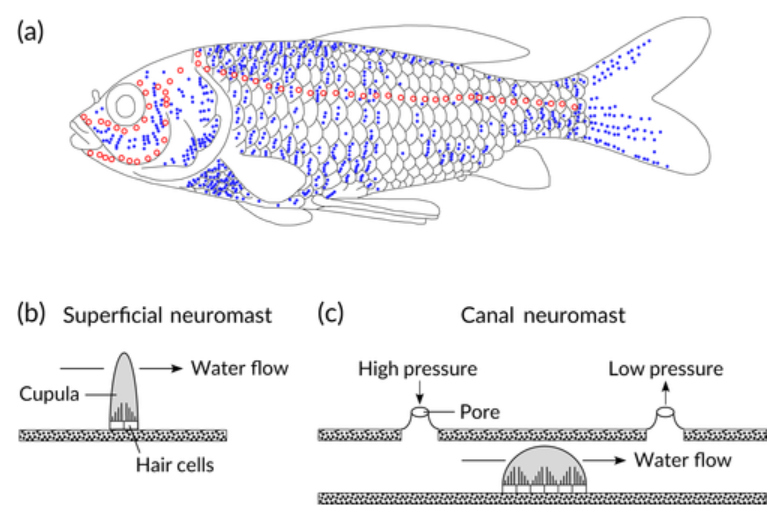
\includegraphics[width=0.49\columnwidth]{figures/Figure3.png}
\end{center}
\caption{(a) Basic anatomy of a lateral line in fish, where blue dots represent SNs and pink circles represent pores of the canal network. (b) Diagram of an SN. (c) Diagram of a CN \citep{Mogdans2018}.}
\label{fig:app:Lat Line}
\end{figure}

\subsubsection{Lateral Line Uses} \label{Lateral Line Uses}

	The lateral line allows fish to detect flow characteristics and collect information about their surroundings that are undetectable by visual or acoustic means. By detecting acute pressure and velocity changes, the lateral line enables fish to ‘feel’ objects that are several body lengths away, track prey by their wake \citep{Montgomery1995}, school with other fish, align with the local current \citep{Montgomery1999}, and adjust their gait for more efficient swimming in the presence of periodic flow \citep{Liao2003}. A particularly telling testimony to the effectiveness of lateral lines are the lifestyles of blind \citep{Windsor2010} and abyss-dwelling fish, which have been observed tracking prey and sensing obstacles with a spatial resolution of 1 mm \citep{Hassan1986}. The lateral line's ability to sense the presence of structures and flow characteristics without the fish's body coming in direct contact with them has come to be known as 'touch at a distance' \citep{Dijkgraaf1962}. 
	
	The lateral line enables fish to take advantage of wakes in the water to swim more efficiently. One such wake is the Karman vortex street, which is described in Section \ref{Karman Vortex Streets}. As \citep{Liao2003} observed, trout placed in a cylinder’s Karman vortex street detected the vortices’ positions and shedding frequency. The fish then adjusted their gaits to match the vortex shedding frequency and swam 180° out of phase with the vortex street, resulting in decreased muscle activity and, therefore, lower energy consumption. This behavior is depicted in a series of frames in \Fref{fig:app:Slalom}. Because the vortex wake was entirely invisible, the fish must have felt the flow characteristics and responded with a behavior that increased swimming efficiency \citep{Liao2003}.

\begin{figure}
\begin{center}
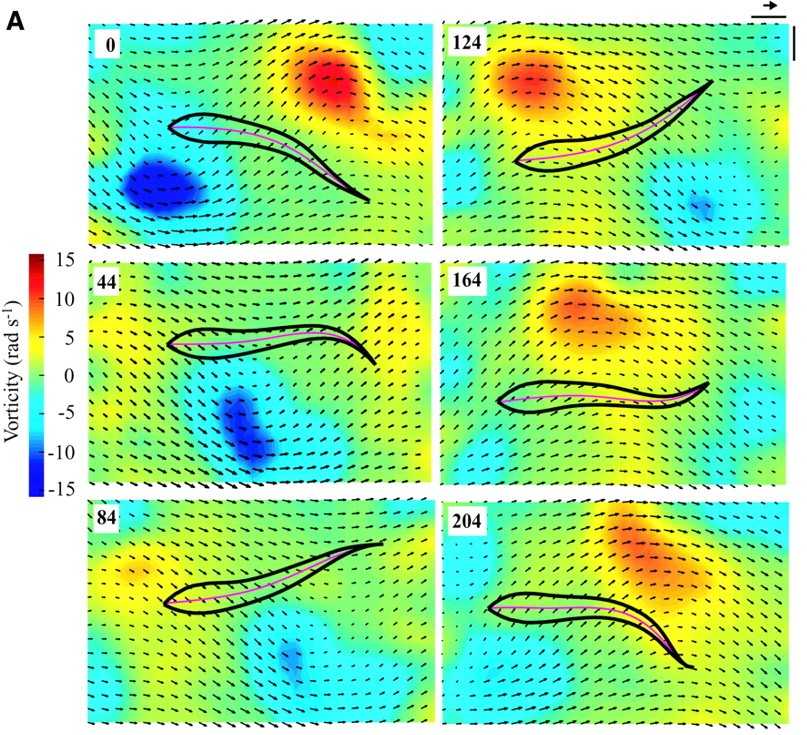
\includegraphics[width=0.49\columnwidth]{figures/Liao Slalom.jpg}
\end{center}
\caption{Bird's-eye view of a trout body outline slaloming through a Karman vortex street. The flow field was created with particle image velocimetry, and subplots are ordered sequentially proceeding from top to bottom on the left, then top to bottom on the right \citep{Liao2003}.}
\label{fig:app:Slalom}
\end{figure}

\subsection{Biological Inspiration}
    
    The slaloming behavior demonstrated by trout and the knowledge that fish fins induce similar vortices in their wake has spurred underwater robotics research to study and create control systems that utilize similar lateral line sensors to achieve more efficient or effective swimming in unmanned underwater vehicles (UUVs). Fish have already demonstrated that pressure-based control loops can be used to swim more effectively, and a lateral line sensing mechanism can provide the wake feedback necessary to develop effective tandem fin propulsion. The overarching theme of this project is to draw inspiration from the propulsion and wake sensing systems observed in nature to develop a control loop for an underwater propulsion system. 
\section{Previous Work}

    Previous researchers have worked to understand and replicate the phenomena described in Section \ref{Natural Systems} in the laboratory environment. They have laid the groundwork for the current project by investigating the fields of vortex sensing with lateral lines and tandem foil wake interaction. To the knowledge of the current team, no previous work has ever applied lateral line technology to a tandem fin control system, and this possibility would link the work of previous researchers to more effective control systems.

\subsection{2D Wake Interaction} \label{2D Wake Interaction}

    Although fish fins are flexible and three dimensional, simplifying their interactions by considering 2D rigid systems composed of their cross sections has allowed for experimental analysis of their wake interactions. Three coherent modes of wake interaction have been observed between flapping foils: constructive, destructive, and vortex pairing \citep{Gopalkrishnan1994}. When foils are phase shifted such that like-rotating vortices meet at the trailing edge of the downstream foil, the vortices build constructively into a single, larger vortex. The two foils create one vortex street with increased circulation. When foils are phase shifted such that oppositely rotating vortices meet, the vortices combine destructively, resulting in dramatically decreased circulation. The resultant vortex street is of the same shape as the vortex street for a single foil, but with reduced circulation. When the foils are not in such a phase that would cause one of the wakes above, the shed vortices meet and pair downstream of both foils and create a double street wider than the street from a single foil \citep{Gopalkrishnan1994}.

\subsubsection{Effects of 2D Wake Interaction} \label{Effects of 2D Wake Interaction}

    Due to the complex fluid dynamics equations governing the wake interactions between flapping foils, the effects of wake interaction have been largely studied through experimental means \citep{Boschitsch2014}. The wake interaction directly impacts the thrust and power coefficients on the trailing foil, with the largest coefficients associated with constructive vortex interactions and the lowest coefficients associated with destructive interactions \citep{Gopalkrishnan1994, Boschitsch2014, Muscutt2017}. Additionally, the foil spacing also influences the vortex interaction. When the spacing between two foils is greater than one half of their chord length, the wake interaction has negligible impact on the dynamics of the upstream foil \citep{Boschitsch2014}.

\subsubsection{Parameters Governing 2D Wake Interaction} \label{Parameters Governing 2D Wake Interaction}

    The degree of wake interaction is dependent on the phase difference between the foils, the Strouhal number, and the foil spacing \citep{Boschitsch2014, Muscutt2017}. These parameters dictate the mode of wake interaction between the foils, as well as the strength of their impact on the coefficients of thrust and power on the downstream foil, which can be observed in \Fref{fig:PW:Thrust vs Phase}. This figure compares the coefficients of thrust, \(C_T\), and power, \(C_P\), for a single fin with those of a downstream fin in a tandem configuration. As the lighter regions indicate, various combinations of phase difference, $\phi$, between tandem fins and the fins' spacing, \(\frac{s}{C}\), cause large improvements in downstream foil performance, e. g. $C_T^*$ at $\frac{s}{C}=1.5$ and $\phi=\frac{7\pi}{4}$. \citep{Boschitsch2014} used foils that only made pitching motions to create \Fref{fig:PW:Thrust vs Phase}, but similar results also occur for foils that pitch and heave \citep{Gopalkrishnan1994, Muscutt2017}.

\begin{figure}
\begin{center}
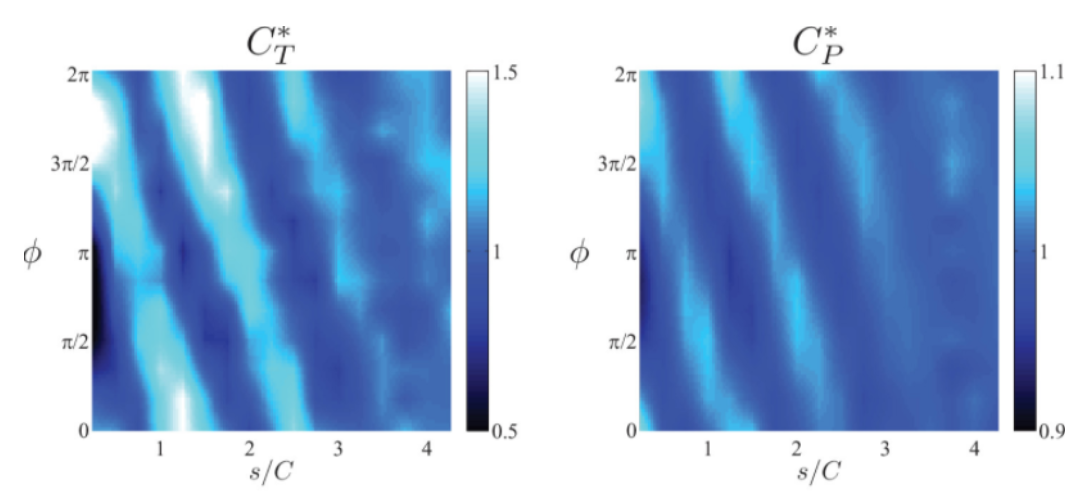
\includegraphics[width=0.8\columnwidth]{figures/Bos Results.png}
\end{center}
\caption{Variation of normalized thrust coefficient (left) and power coefficient (right) on a downstream foil with respect to phase difference in radians, \(\phi\), and foil spacing in units of foil chord lengths, \(s/C\). The coefficients are normalized by dividing by the coefficients experienced by a single flapping foil under the same parameters, as \(C_T^*=\frac{C_{single foil}}{C_{tandem foil}}\). Lighter regions indicate parameter combinations that offered improved characteristics relative to a single flapping foil, and darker regions indicate combinations that decreased characteristics \citep{Boschitsch2014}.}
\label{fig:PW:Thrust vs Phase}
\end{figure}

% Cam 12/29: talk about specific numbers of thrust improvement? Take a paragraph to explain why it's valuable to control the wake interaction? Should this paragraph be placed later in the proposal?

\subsection{Human Made Lateral Lines} \label{Human Made Lateral Lines}
 
    Several groups have developed artificial canal neuromasts using microelectromechanical systems (MEMS) \citep{Fan2002, Chen2007, Kottapalli2014} , or optical sensors \citep{Klein2011}. However, because CNs detect pressure differences across the surface of fish, many researchers have implemented off-the-shelf pressure sensors to achieve similar effects \citep{Venturelli2012} \citep{DeVries2015} \citep{Zhang2015}. These configurations eliminate the need for a canal, as the differential pressure between two points can be calculated by simply subtracting the measurements from adjacent sensors. The lateral lines become linear arrangements of sensors, such as the arrays built by \citep{Venturelli2012} and \citep{Fernandez2011}, shown in \Fref{fig:PW:Human Lateral Lines}. The sensors are embedded in a structure and make contact with the water through holes in the surface.

\begin{figure}
\begin{center}
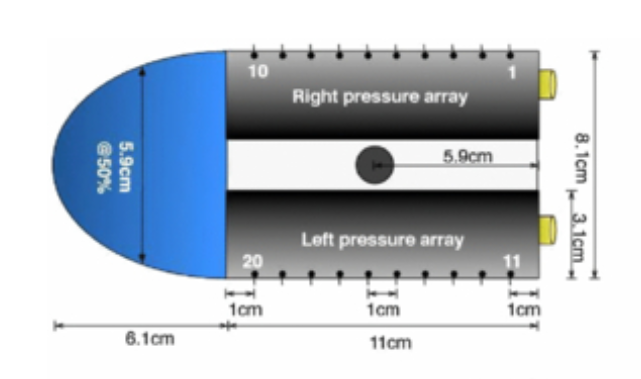
\includegraphics[width=0.60\columnwidth]{figures/Venturelli Setup.png}
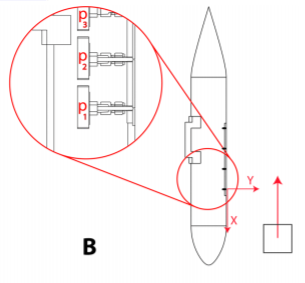
\includegraphics[width=0.30\columnwidth]{figures/Fernandez Setup.png}
\end{center}
\caption{Linear pressure sensor array designed to detect oncoming vortices using absolute pressures, where each black dot represents an MS5401-BM pressure sensor (left) \citep{Venturelli2012}. Linear array of Honeywell 19C015PG4K pressure sensors used for classifying nearby objects (right) \citep{Fernandez2011}.}
\label{fig:PW:Human Lateral Lines}
\end{figure}

\subsection{Vortex Wake Feature Extraction with Lateral Lines} \label{Vortex Wake Feature Extraction with Lateral Lines}

    Pressure sensor arrays have demonstrated the ability to draw both qualitative and quantitative characteristics from object wakes. As described in Section \ref{Karman Vortex Streets}, vortices produce low pressure regions in the water. These vortex streets create perceptible undulations in the readings from differential pressure sensor arrays, as can be seen in \Fref{fig:PW:Venturelli Results}. This pressure data was generated by \citep{Venturelli2012} when they placed the array shown in \Fref{fig:PW:Human Lateral Lines}(left) behind a cylinder in steady flow. The vortices, represented by the alternating bands of red and blue, have both a time and magnitude associated with them. The time measured between vortices allows for calculation of the oscillation frequency, while the time one vortex takes to reach a sensor of a known distance away allows for calculation of the flow speed. In \Fref{fig:PW:Venturelli Results}, this is visible in the diagonal shape of the red and blue bands, as the vortices are measured by each sensor as they are advected downstream by the underlying uniform flow. Downstream sensors detect vortices later than upstream units. The flapping frequency observed by the sensors is apparent at any perpendicular displacement from the vortex street, as seen in \Fref{fig:PW:Chambers Results}, although the signal to noise ratio decreases as the sensor array makes less contact with the vortices \citep{Chambers2014}. \Fref{fig:PW:Chambers Results} also shows that the frequency perceived by a sensing array is constant when its movement within the street is small, as moments where frequencies peaked occurred at moments when the array was moving fastest \citep{Chambers2014}.  In the case of flapping foils, the vortex shedding frequency, \(f_h\), and free stream flow speed, \(U_\infty\), are two of the three terms related to the Strouhal number, according to \ref{Eq:Fin St}. This Strouhal number corresponds directly to the efficiency, thrust, and power of the foil. As shown by these studies, linear pressure sensor arrays have the potential to indicate the effective Strouhal number of a system and, thus, offer real-time feedback on the performance of a system. 
    
    While the artificial lateral line response to a single Karman vortex wake is well documented, no studies to date have characterized its response in the presence of two interacting vortex wakes. This research project will perform experiments to understand how these sensors would perceive such a wake.
% how to say that the frequency reading is robust as long as the sensor array is still?
\begin{figure}
\begin{center}
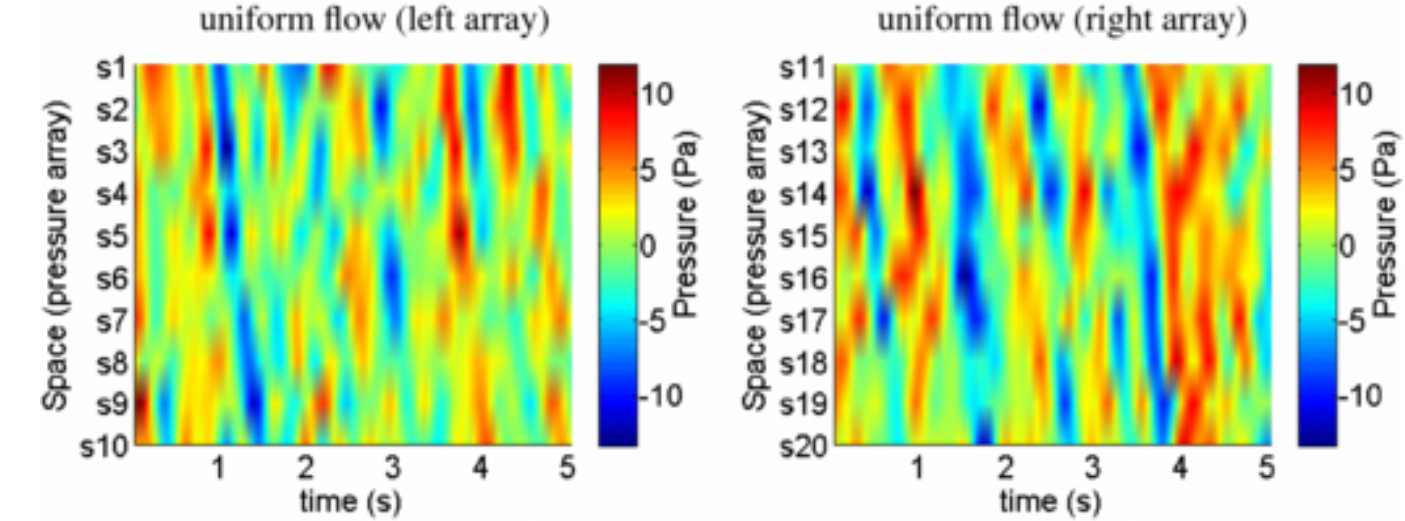
\includegraphics[width=0.80\columnwidth]{figures/Venturelli Readings.PNG}
\end{center}
\caption{Pressure readings from each sensor on the artificial lateral line shown in \Fref{fig:PW:Human Lateral Lines}(left). Higher numbered sensors on the same plot are farther downstream than the lower numbered sensors. Pressure readings are encoded by color and correspond to the vortices shed by an upstream cylinder \citep{Venturelli2012}.}
\label{fig:PW:Venturelli Results}
\end{figure}
\begin{figure}
\begin{center}
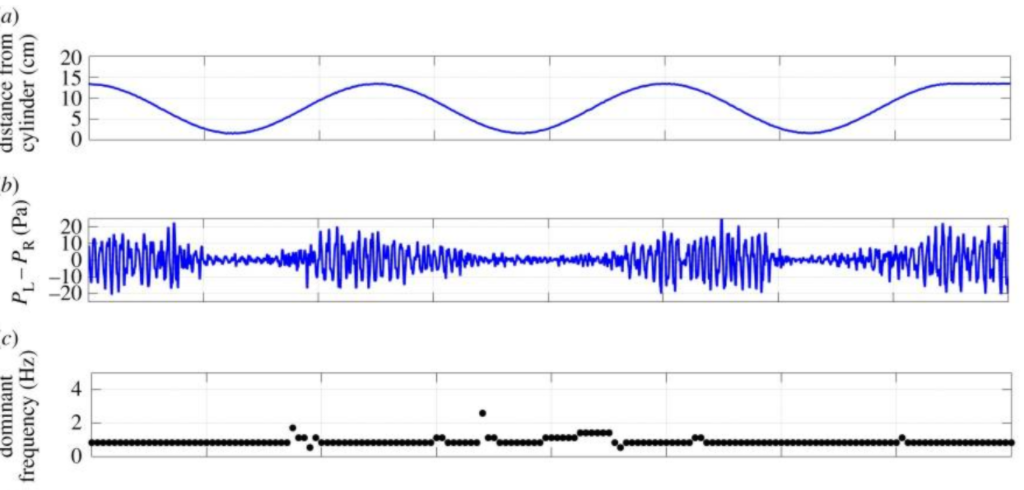
\includegraphics[width=0.80\columnwidth]{figures/Chambers Lateral Results.PNG}
\end{center}
\caption{A pressure sensing array's lateral displacement from a Karman vortex street with respect to time (top). Differential pressure readings between the left and right sides of an array as it moved into and out of the vortex street (middle). The dominant frequency observed at each moment in the array's path (bottom) \citep{Chambers2014}.}
\label{fig:PW:Chambers Results}
\end{figure}

    Lateral line-inspired systems consisting of commercially available pressure sensors have demonstrated the ability to detect wake characteristics with an accuracy that enables object identification based solely on the pressure readings. The work of \citep{Fernandez2011} shows one example of this. When either a square or circular cylinder passed alongside the sensor array shown on the right side of \Fref{fig:PW:Human Lateral Lines}, the pressure sensors would generate pressure waves such as those shown in \Fref{fig:PW:Square vs Circular Profiles}. The two types of cylinders produced distinct waves, from which \citep{Fernandez2011} derived salient features that determined the contour of the cylinder with only 1.2\% error.
% Cam: Is this picture adding anything to the conversation?
\begin{figure}
\begin{center}
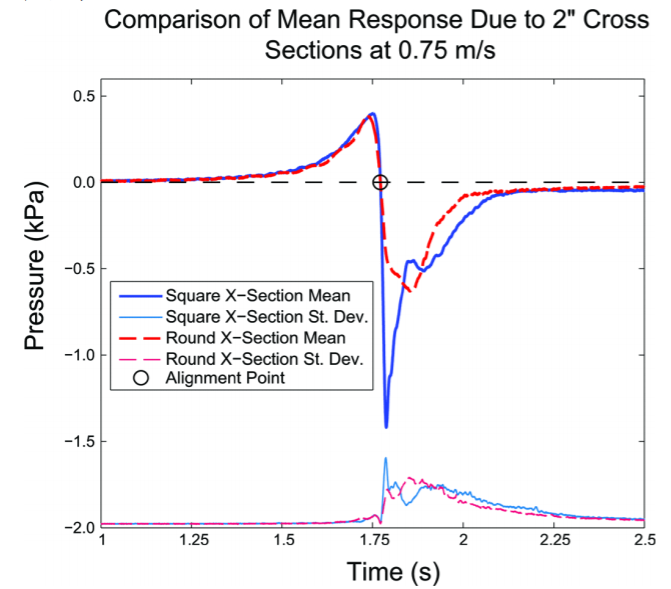
\includegraphics[width=0.50\columnwidth]{figures/Fernandez Results.png}
\end{center}
\caption{Average pressure response for square and circular cylinders, with the standard deviation offset by -2.0 kPa \citep{Fernandez2011}.}
\label{fig:PW:Square vs Circular Profiles}
\end{figure}

%\subsection{Tandem Foil Simulation with Lily Pad} \label{CFD Attempts}

    %Due to the complex equations governing vortex interactions, flow calculations are often performed using computational fluid dynamics software. Lilypad is an open source CFD program developed by Dr. G Weymouth for quick, 2D flow simulations \citep{Weymouth2015}. It solves the Navier-Stokes equations and applies body boundary conditions over surfaces using the Boundary Data Immersion Method, while maintaining a Cartesian grid for calculations \citep{Weymouth2011}. \citep{Muscutt2017} simulated tandem flapping foils using Lily Pad in order to find the effective coefficients of thrust, power, and efficiency on the downstream foil for multiple phase shifts and foil spacings. The chief benefit of fast running computational software is that a plethora of trials can be run in a fraction of the time required to run a physical test, while varying the experimental parameters with a set of keystrokes. The differential pressures between any two points can be calculated in real time for each trial and produce theoretical results for comparison to a physical model.

% This method convolves the equations governing the simulation using a kernel, creating the update equation for the convoluted velocity, \(\vec{u_e}\), and the update equation for the velocity divergence, given as
% \[\vec{u_e} =\mu_0\vec{f}+(1-\mu_0)\vec{b}+\mu_1\frac{\partial}{\partial n}(\vec{f}-\vec{b})\]
% \[\vec{\nabla}\cdot\vec{u_e}=(1-\mu_0)\vec{\nabla}\cdot\vec{b}-\mu_1\frac{\partial}{\partial n}(\vec{\nabla}\cdot\vec{b})\]
% where  
\section{Project Goals}

    Based on the qualities observed in nature and the state of current research, this project will target a set of primary and secondary objectives. The primary objectives will serve as the priority in the event of setbacks.

\subsection{Primary Objectives}
\begin{itemize}
    \item Identify numeric characteristics of tandem fin vortex wakes that can be observed using an artificial lateral line.
    \item Infer a relationship between measured vortex wake traits and tandem fin phase difference.
\end{itemize}
\subsection{Secondary Objectives}
\begin{itemize}
    \item Investigate a low cost lateral line sensing mechanism for wake detection.
    \item Determine the best measured wake trait for phase angle estimation.
    \item Expand USNA's capability for lateral line sensing.
\end{itemize}

\section{Materials and Methods}

    This project will use an artificial lateral line to observe the vortex interaction between 2, two dimensional, tandem flapping foils in USNA's Large Re-Circulating Water Tunnel. First, the commercially available pressure sensors at USNA will be evaluated to determine which is optimal for wake observation based on a predefined set of standards. Next, the identified sensor will be built into an artificial lateral line as inspired by \citep{Venturelli2012}. Then, the sensor array's response to a single vortex street will be analyzed by placing it downstream from a single flapping foil, similar to the initial experiments conducted by \citep{Venturelli2012} and \citep{Boschitsch2014}. Finally, the sensor array will be placed downstream from two, tandem foils flapping at various phases. The data collected from this experiment will be analyzed in MATLAB for features that correlate with the phase difference.

\subsection{The Sensor Array} \label{The Sensor Array}
\subsubsection{Pressure Sensor Characterization} \label{Pressure Sensor Characterization}
     
    Before building an artificial lateral line, it will be necessary to identify and characterize the best available pressure sensor. All sensors are influenced by high frequency noise and low frequency bias drift. While filters can be implemented to minimize the effects of noise, the vortex interactions caused by the tandem fins will register as somewhat high-frequency pressure changes to the sensors, so only a high-pass filter will be created and used to mitigate bias drift. The USNA Hydromechanics Laboratory currently possesses several pressure sensors relevant to this work, and the sensors used in \citep{Venturelli2012} and \citep{Chambers2014} are also readily available.
    
    The Hydromechanics Laboratory's available sensors will be tested and evaluated based on their sampling frequency, noise, bias drift, and sensitivity. The most desirable trait will be low noise, as a higher signal to noise ratio will enable more accurate and consistent readings. The sensors' sensitivities are second most important, as they are the second component of the sensors' signal to noise ratios. The sampling frequency is third most important, as a higher frequency will allow the array to sense vortices that are close together. The bias drift is least important, as it can be largely compensated for using a high-pass filter and calibration.
    
    Each sensor will be mounted to a PVC pipe in stationary water and their data will be collected through their respective interfaces. The sensors' outputs will be recorded for multiple trials, each lasting several minutes. The resultant data will provide information on each sensors' bias drift frequency, which can be eliminated using a high-pass filter of the form
    \begin{equation} \label{Eq:High pass filter}
    x_n=\frac{2-aT}{2+aT}x_{n-1}+\frac{2}{2+aT}(y_n+y_{n-1})
    \end{equation} 
    where \(x_n\) and \(x_{n-1}\) are the current and previous output reading, respectively, \(y_n\) and \(y_{n-1}\) are the current and previous input readings, respectively, \(T\) is the sampling period, and \(a\) is the bias drift frequency found for a sensor. The sampling period is related to the sampling frequency by \(T=\frac{1}{f}\). Applying this filter to each trial's data will leave only high frequency noise for each sensor.
    
    The impact of this noise is directly related to the standard deviation in a given sensor's pressure readings over the trial, as the sensors should ideally measure a single value. Sensors with higher standard deviations will show the highest degree of noise, and this will factor into their selection for use in the lateral line.

%\begin{figure}
%\begin{center}
%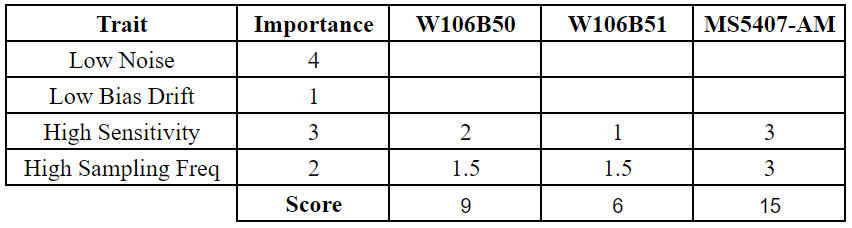
\includegraphics[width=0.8\columnwidth]{figures/Decision Matrix.png}
%\end{center}
%\caption{Decision matrix used to compare the available pressure sensors.}
%\label{fig:methods:Decision Matrix}
%\end{figure}

\subsubsection{Constructing the Sensor Array} \label{Constructing the Sensor Array}
    
    The optimal sensor model identified in Section \ref{Pressure Sensor Characterization} will be built into an artificial lateral line. The sensors will be arranged into two rows inside a PVC tube, positioned on opposite sides of the tube and extending from one end to the other. A cross section of the anticipated layout is shown in \Fref{fig:methods:2D Setup}. The sensors will make contact with the water through pre-drilled holes that are evenly spaced. Their pressure data will be carried through the tube and out its downstream end via coaxial cables. The data will be exported to a laptop computer and analyzed in MATLAB. Several sensors will be used, likely within the range of 8-16 units, depending on the interface required.
    
\subsection{Foil Construction and Actuation} \label{Foil Construction and Actuation}
    
    The foils will be made with a NACA0016 cross section and a chord length, \(C\), of 8 cm. The bodies will be fabricated in the Rickover Model Shop using foam and aluminum. A rod will be placed along the pitch axis, located one quarter chord behind the leading edge. The foil setup will resemble that of \citep{Boschitsch2014}, enabling quick data comparison. The NACA0016 foil will lend itself to better inferences from  data, as its characteristics are well documented and understood. The foils will be 0.40 m tall, spanning the height of the Re-Circulating Water Tunnel. 
    
    The foil movements will be programmed with an Mbed microprocessor, and they will be actuated by servomotors from previous bio-inspired propulsion experiments in the Biomechanics Laboratory. To make this project attainable using USNA equipment, the foils will not undergo heave motions, and will only pitch. This motion will still achieve the necessary vortex interactions that highlight thrust generation as a function of the foils' phase difference. The foil cross sections and a sketch of the 3D setup can be found in \Fref{fig:methods:2D Setup} and \Fref{fig:methods:3D Setup}, respectively. When placed in tandem, the foils will move according to the equations given in \Fref{tab:methods:EOM}.
\begin{center}
\begin{table}
\caption{Equations of Foil Motion}
\label{tab:methods:EOM}
\begin{tabular}{ccc}
\toprule
Motion & Upstream Foil & Downstream Foil \\ 
\midrule
Pitch & \(\theta(t)=\theta _msin(\omega t)\) & \(\theta (t)=\theta _msin(\omega t+\phi)\) \\
\end{tabular}
\end{table}
\begin{figure}
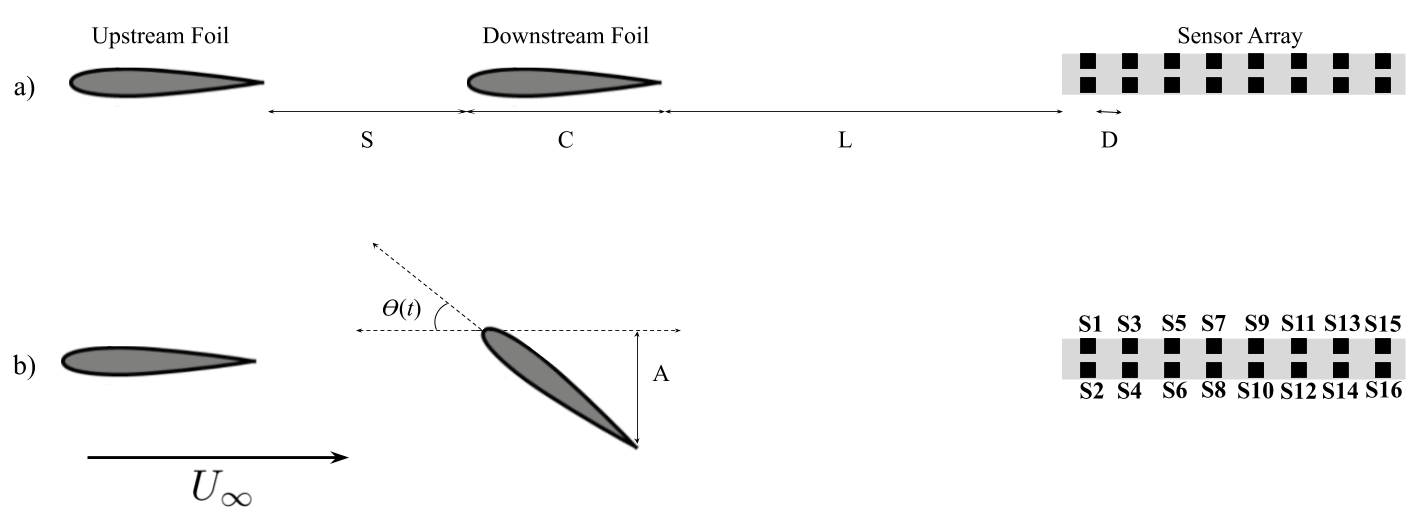
\includegraphics[width=0.8\columnwidth]{figures/Experimental Setup.png}
\caption{Stationary depiction of 2D tandem foil experiment setup with foil spacing, chord length, and sensor spacing marked (a). 2D tandem foils in motion with foil pitch angle, stroke amplitude, and free stream velocity marked (b).}
\label{fig:methods:2D Setup}
\end{figure}
\begin{figure}
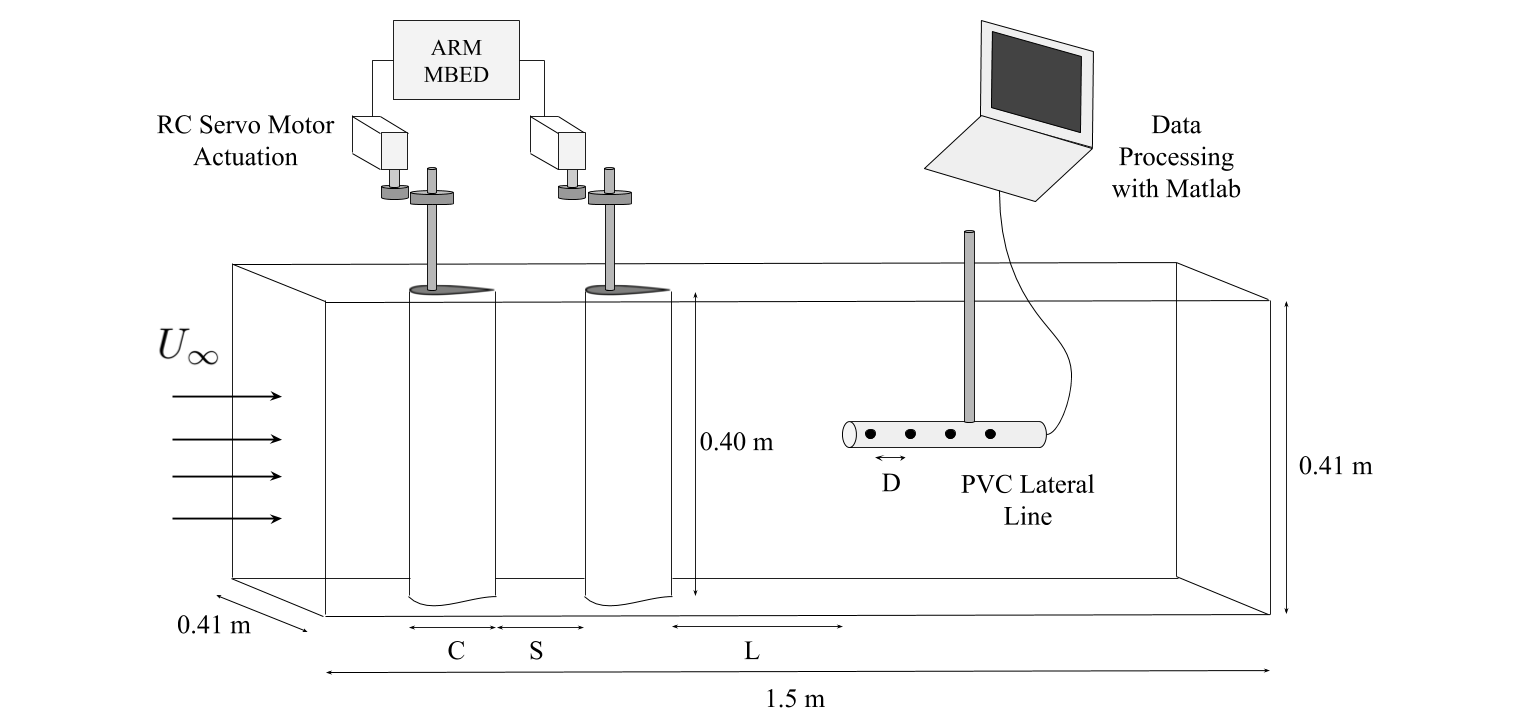
\includegraphics[width=0.95\columnwidth]{figures/3D Tank Setup.png}
\caption{3D depiction of experimental setup with free stream velocity, \(U_\inf\), foil chord, $C$, foil spacing, $S$, distance between the foils and lateral line, $L$, and the spacing of pressure sensors, $D$, marked. The tank dimensions and foil height are also given.}
\label{fig:methods:3D Setup}
\end{figure}
\end{center}

\subsection{Single Foil Test} \label{Single Foil Test}
    
    It will be necessary to study the lateral line's response to a single vortex wake before applying it to tandem foil vortex wakes. This will allow for calibration of sensors and verification of the setup's accuracy, as results can be compared to previous work. This experiment will also determine the best experimental parameters for vortex observation and demonstrate the lateral line's sensitivity to vortex location. In doing so, it will replicate the primary experiments from \citep{Venturelli2012} and \citep{Chambers2014}, as well as the initial test by \citep{Boschitsch2014}. The lateral line constructed in Section \ref{The Sensor Array} will be placed two chord lengths downstream from one foil constructed in Section \ref{Foil Construction and Actuation}, located in the Large Re-Circulating Water Tunnel. This setup is identical to that shown in \Fref{fig:methods:3D Setup}, but the upstream foil is omitted. The trial will begin with the fin at rest for five seconds, the fin will flap for five oscillation cycles, and then it will come to rest for ten seconds. The differential pressure readings between opposite sensors (i.e. s1-s2, s3-s4 in \Fref{fig:methods:2D Setup}) will be collected and analyzed in MATLAB. The average pressure observed during the rest periods will allow for sensor calibration and show if any sensor drift was present during the trial.
    
\subsubsection{Determining Fin Motion Parameters} \label{Determining Fin Motion Parameters}
    
    Several trials will be conducted to determine the optimal fin motion parameters for vortex detection. The fin's Strouhal number will be fixed at 0.25, a relevant value for finned propulsion discussed in Section \ref{Fin Propulsion}. The peak edge displacement, \(A\), free stream velocity, \(U_\inf\), and maximum pitch angle, \(\theta_m\), will be varied until the lateral line's detects the vortices in a similar manner to those in \Fref{fig:PW:Chambers Results}. During this experimentation, the Reynolds number does not need to be matched for an actual fish, as vortex shedding and wake interaction is known to be largely independent of Reynolds number. The motion parameters used in \citep{Boschitsch2014} will provide a starting point for this experimentation. Additionally, this test will help to determine the optimal distance between the foil and lateral line for vortex detection. This value is marked as $L$ in \Fref{fig:methods:2D Setup} and \Fref{fig:methods:3D Setup}.
    
\subsubsection{Testing Lateral Sensitivity} \label{Testing Lateral Sensitivity}
    
    Once the vortex street is consistently perceived, the lateral line will be moved out of the direct path of the vortex wake. This should display characteristics similar to those in \Fref{fig:PW:Chambers Results}, where the sinusoidal vortex signals decreased in amplitude with lateral distance. This step will demonstrate the lateral line's sensitivity to vortex displacement.

\subsection{Tandem Fin Test} \label{Tandem Fin Test}

    After completing baseline tests with a single foil, this project will collect wake data from a tandem foil setup at multiple phase differences. A second foil will be added to the setup described in Section \ref{Single Foil Test}, completing the construction of the sketch in \Fref{fig:methods:3D Setup}. This foil will be positioned upstream of the single foil with a spacing, \(S\), of one chord length, so that the downstream foil will not influence its vortex production \citep{Boschitsch2014, Muscutt2017}. The system will be placed under a constant, uniform flow using the Re-Circulating Water Tunnel's four-bladed axial flow impeller. A series of about twenty-five tests will be conducted where the tandem fins will flap according to the equations given in \Fref{tab:methods:EOM}. Their phase difference, \(\phi\), will differ for each trial and range from 0 to 180°. Each trial will begin with the foils at rest for 5 seconds, the fins will flap for five cycles, and then they will come to rest for ten additional seconds. The pressure readings during the stationary portion of the trial will show the noise and unperturbed water pressure. The constant pressure reading over the last ten seconds will indicate any bias in the pressure readings over the course of the experiment. Three trials will be run for each \(\phi\), yielding a total of seventy-five trials. The differential pressure data will be saved for further analysis described in Section \ref{Data Analysis}.
    
\subsection{Materials}

    The sensors and their interface materials are available through the Hydromechanics Laboratory, while the PVC tubing and its mount are available through the Rickover Model Shop. The foil bodies will be constructed with aluminum and foam in the Model Shop, while the servomotor actuators for the foils will be reused from past independent research projects within the Biomechanics Laboratory. All experiments will take place in the Large Re-Circulating Water Tunnel located in the Hydromechanics Laboratory, whose dimensions are 0.41 m x 0.41 m x 1.50 m.
    
%\subsection{Optional Fluid Simulation}

%    If the experimental procedures and data analysis described above are completed with significant time remaining, an additional objective will be to validate experimental computational fluid dynamics (CFD) models. As described in Section \ref{CFD Attempts}, the Boundary Data Immersion Method (BDIM) has offered a potential route for simulating fluid dynamics in the presence of multiple moving bodies, such as tandem fins. The experimental data developed for this project could be used to validate BDIM-based CFD programs in OpenFoam and Lilypad by running the simulated versions of the trials and comparing the actual and simulated downstream pressures. These CFD methods will take significant time to learn, and this objective will only be pursued if the project is two months ahead of schedule. 
\section{Data Analysis} \label{Data Analysis}
\subsection{Single Foil Data} \label{Single Foil Data}

    The procedure described in Section \ref{Single Foil Test} serves as a way to test the flapping foil and lateral line. Any detected sensor bias drift will be recorded and accounted for using the high pass filter given in (\ref{Eq:High pass filter}). The data will then be analyzed using a Fourier Transform to determine the dominant frequency of the vortex wake, which should be identical to the foil's flapping frequency. Other dominant frequencies may indicate frequencies characteristic of the actuation mechanism or tank; identifying them during this phase will allow them to be eliminated in subsequent experiments. In addition, the phase difference between inline sensor pairs (s1-s3, s2-s4) will be used to calculate the distance between vortices. Based on the expected results, the known distance between sensors, \(D\), and the time of maximum differential pressure readings allows the freestream velocity to be calculated with \(\frac{D}{t_2-t_1}=U_\infty\). The calculated \(U_\infty\) should agree with the value programmed into the water tunnel. The estimated \(U_\infty\) and time between successive vorticity peaks allow the distance between vortices and the shedding frequency to be calculated.
    
\subsection{Tandem Foil Data} \label{Tandem Foil Data}

    The previous sections have collected a host of pressure data that corresponds to known phase differences between flapping foils. This section will seek to find relationships between them by experimenting with a variety of algorithms and features. The tandem foil wake data will be analyzed for salient features that correlate with phase difference. While previous works point to a set of features that will be strong leads, the researchers will scan the recorded data and experiment with new traits. Based on the previous studies, the lateral line's pressure signature should hold features that can be used to infer the tandem fins' phase difference. Several methods will be used to identify this relationship.
    
% "Based on previous studies, we expected salient features of vortex interaction in the artificial lateral lines array's pressure signature."

\subsubsection{Expected Tandem Wake} \label{Expected Tandem Wake}
    
    Based on the 2D wake interaction modes described in Section \ref{2D Wake Interaction}, for a majority of preset fin phase differences, \(\phi\), the fin vortices are expected to form loose pairs and drift away from the center line. For a small window of \(\phi\) the vortices will combine either constructively or destructively. In the pairing case, the lateral line is likely to perceive each individual vortex as a local maximum differential pressure, and, as seen in \citep{Chambers2014}, the distance of the vortex from the lateral line will correspond directly with the magnitude of this local maximum. The distance between each vortex in a pair can be found using the method described in Section \ref{Single Foil Data}. Based on this data, the lateral line can identify the degree of pairing between two vortices.
    
    For constructive or destructive vortex interaction, the vortices are expected to remain on the wake's center axis. The presence of significantly increased vorticity and, therefore, decreased pressure will identify constructive interaction, while decreased vorticity and a smaller differential pressure will identify destructive interactions.
    
\subsubsection{Expected Features} \label{Expected Features}
    
    Based on the previous work and discussion in Section \ref{Expected Tandem Wake}, a number of features should offer insight on the tandem fins' phase difference.
    
    The Fourier Transform will identify dominant frequencies for each trial. While a single vortex wake and constructive or destructive tandem wakes will produce a single frequency identical to the foils' flapping frequency, in the presence of multiple paired vortices, the Fourier Transform will translate the distance between vortices into higher frequencies. \citep{Venturelli2012} used the Fast Fourier Transform (FFT) over 3-5 second intervals to calculate the dominant frequencies in a vortex wake, and a similar practice may be applied to the tandem foil data to provide salient frequency domain features.
    
    An additional feature will be the relative perceived intensity of the vortices. As explained in Section \ref{Expected Tandem Wake}, the distance of vortices from the lateral line will vary directly with the magnitude of their pressure signature. Comparing this intensity with the intensity of inline, single vortices can allow a relationship between intensity and relative distance to be developed.
    
    A third promising feature option will be the number of vortices detected over one stroke cycle. Preliminary simulations in Lily Pad, an open source computational fluid dynamics program \citep{Weymouth2015}, suggest that, in addition to paired vortices, many phase differences will also create smaller, unpaired vortices. Examining the pressure data over the course of one stroke cycle and counting the number of local peaks could create another feature that can indicate the phase difference.
    Several other viable features likely exist, and they will be identified by comparing the single foil wake data with the multiple tandem wakes' data.
\subsubsection{Mapping Features to Phase Difference} \label{Mapping Features to Phase Difference}
    
    There are several methods that could map one or all of the features developed in Section \ref{Expected Features} to the tandem fin phase angle. One strategy will be a regression plot with individual features plotted against their corresponding phase angle. Calculating the best fit line for this plot may show a relationship that allows phase angle to be directly calculated based on observed wake features. A fit line's coefficient of determination, \(R^2\), will indicate its accuracy, as this value is indicative of the plotted points' distance from the estimated fit line. The feature that allows the most accurate line of best fit to be drawn will be identified.
    
    Alternatively, several features may be combined at once and related to the foils' phase difference with a Bayesian classifier, decision tree, lookup table, or particle filter. MATLAB contains all of these methods, and they can be employed relatively quickly for cross comparison. Other methods may be tested, but these will serve as a starting point.
\section{Applications}
    
    By identifying numeric characteristics of tandem fin wakes that are observable with a lateral line and relating these characteristics to the fins' phase difference, this project will lay the groundwork for a feedback control loop. 
    
    Tandem fins offer an incredible increase in maneuverability relative to single fin designs, and varying the phase difference between the fins can create nearly doubled thrust \citep{Gopalkrishnan1994, Muscutt2017}. However, in the design of bio-inspired vehicles, open loop programming requires slow, intense calculations of the fluid dynamics around the vehicle and the result is not robust in the face of environmental disturbances, such as collisions, object wakes, and cross currents. A passive feedback mechanism able to estimate the vortex pairing in real time and adjust the foil oscillation phase difference would improve thrust in the presence of disturbances, while also simplifying onboard vehicle trajectory calculations.
    
    The ability to infer upstream behaviors based on observed wake characteristics enables underwater schooling and wake tracking, behaviors that are quite desirable for UUV design. This is especially attractive for naval applications, and the Office of Naval Research is currently funding bio-inspired sensing methods under Code 34.
    
    While previous teams have used artificial lateral lines to detect flow features from external sources, such as obstacles and vortex-producing shapes, this project will be the first work that employs a lateral line in detecting self-generated fluid interactions. This research is novel and holds the potential for significant future experimentation and implementation.
    
    Future teams can build on this research by examining the effects of heave motions, flexible fins, and 3D wakes on the vortex interactions seen by the lateral line. The lateral line built for this project will also enable future USNA teams to investigate 'touch at a distance' for naval vessels.
\section{Risk Management}
    This project has a high likelihood of results due to its simplifications, observed behaviors in nature, and readily available materials.
    
\subsection{Simplifications}
    While the tandem fin system is inspired by biological systems, many of the factors that complicate its study are omitted, which makes the results more consistent and attainable within the Trident timeline. In nature, fins are flexible, have complex 3D shapes, and move with both pitch and heave motions. This project utilizes rigid, 2D foils that only make pitch motions. Previous work has shown that this arrangement still achieves improved thrust and power compared to single fin arrangements, while also creating measurable vortex wakes. These simplifications allow this project to use USNA-built fins and previous foil actuation mechanisms developed in previous projects. This requires less time to be spent on experimental setup, and this time will be reallocated for signal processing.
    
\subsection{Readily Available Materials}
    This project's methods will be easily attainable using USNA's existing resources. All experiments will be conducted in the Large Re-Circulating Water Tunnel, which should not need significant modification before use. The tandem foils can be easily built in the Model Shop using foam and aluminum, but, in the case of setbacks, they can also be made with 3D printers or ordered online in slightly different shapes. The foil actuation mechanisms can utilize materials already under development in the Biomechanics Laboratory. Meanwhile, the lateral line will use sensors that are relatively inexpensive, and the Hydromechanics Laboratory staff has a high degree of familiarity with their use. The data processing tools that will likely be used for this project are readily available in MATLAB with online documentation. The majority of the supplies and expertise for this project's materials and methods are located at USNA, making this project robust against supply chain disturbances and experimental roadblocks.
        
\subsection{Existence of Results}
    As discussed in Section \ref{Natural Systems}, fish have been observed using their lateral lines to achieve desired thrust, power, and efficiency. They sense wake features and adjust their gaits accordingly, demonstrating a real time feedback control loop based on observable wake features. Previous researchers have characterized the wake interactions of tandem foils and the ability for current lateral line technology to determine wake features. The missing link between observed features and tandem fin wake interaction has already been observed in nature, showing that this project's solution exists.
\section{Conclusion}

    This project will enable future teams to design feedback control loops for tandem flapping foils based on their observed downstream effects. To do this, the project will build a lateral line using commercially available pressure sensors and characterize the line's response to a single flapping foil. Then, the line will collect wake data from tandem foils flapping at several phase differences. The resultant pressure data will be analyzed for features that differ with respect to phase difference, and a relationship will be inferred between the features and phase difference. Previous work and readily available tools show that these goals are highly attainable. The ability to infer phase difference between two tandem fins will help future teams to improve underwater agility, conduct UUV schooling, and track objects by their wake.
    
    

\bibliography{trident.bib}
%\usepackage{appendix}
\appendix
\section{Pressure Sensor Data Sheets}

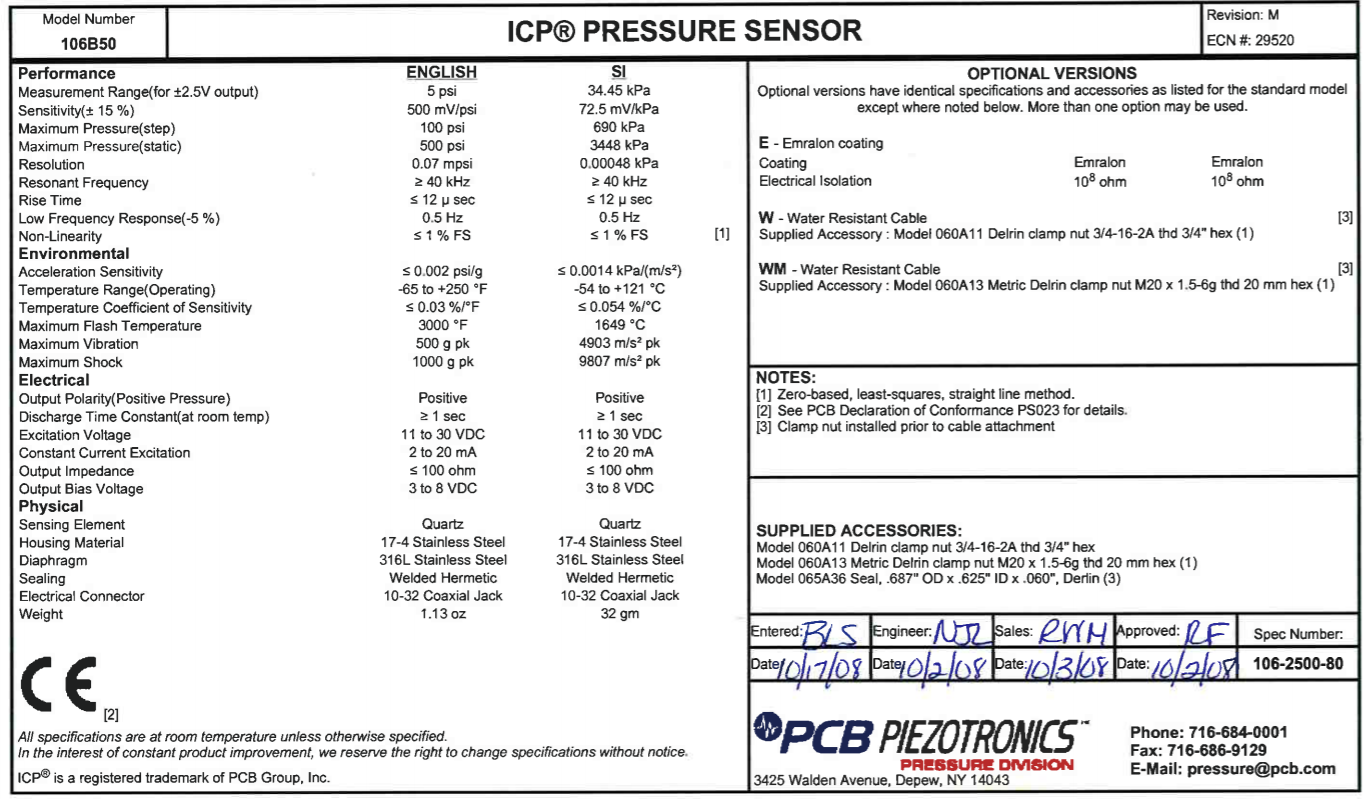
\includegraphics[width=1\columnwidth]{figures/106B50 DS.PNG}
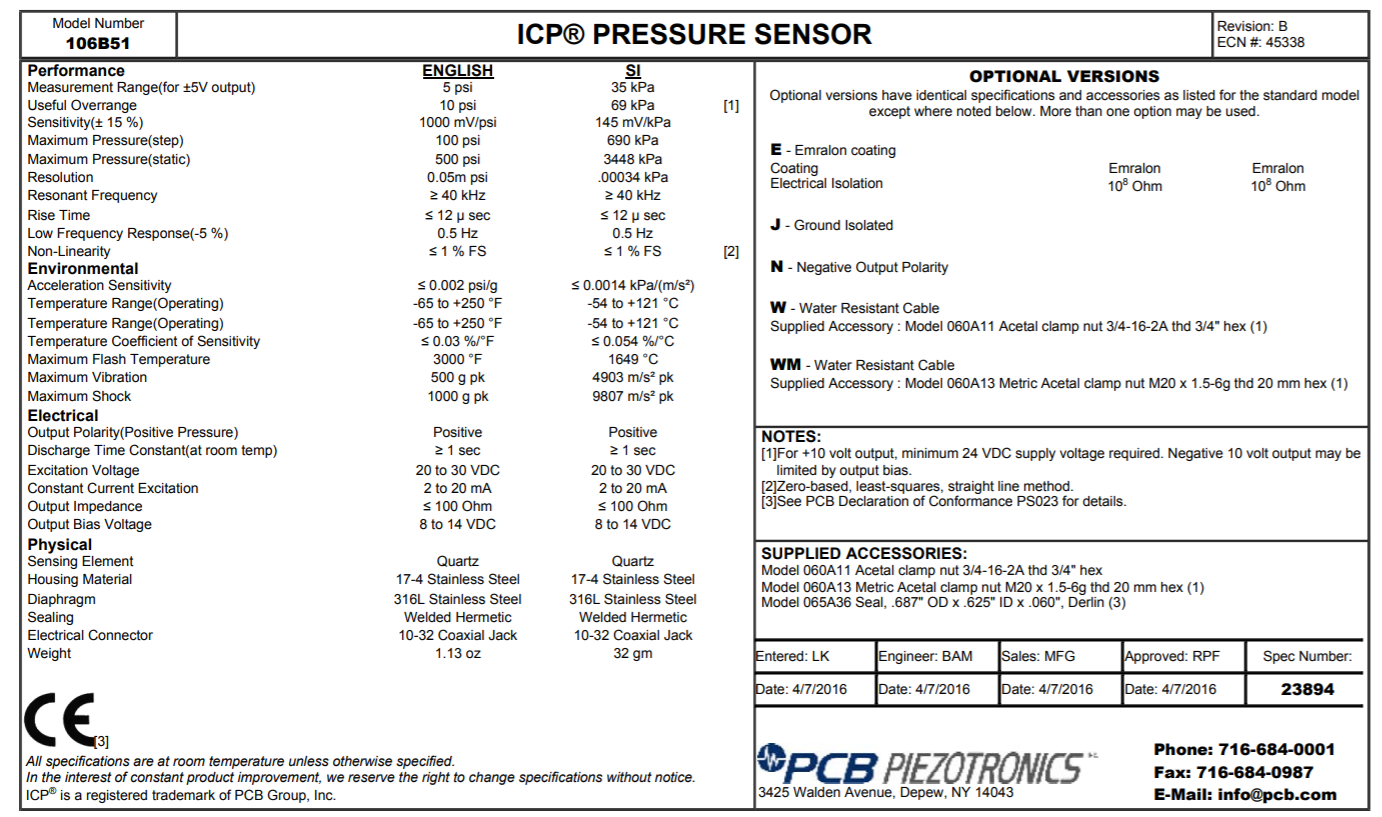
\includegraphics[width=1\columnwidth]{figures/106B51 DS.PNG}
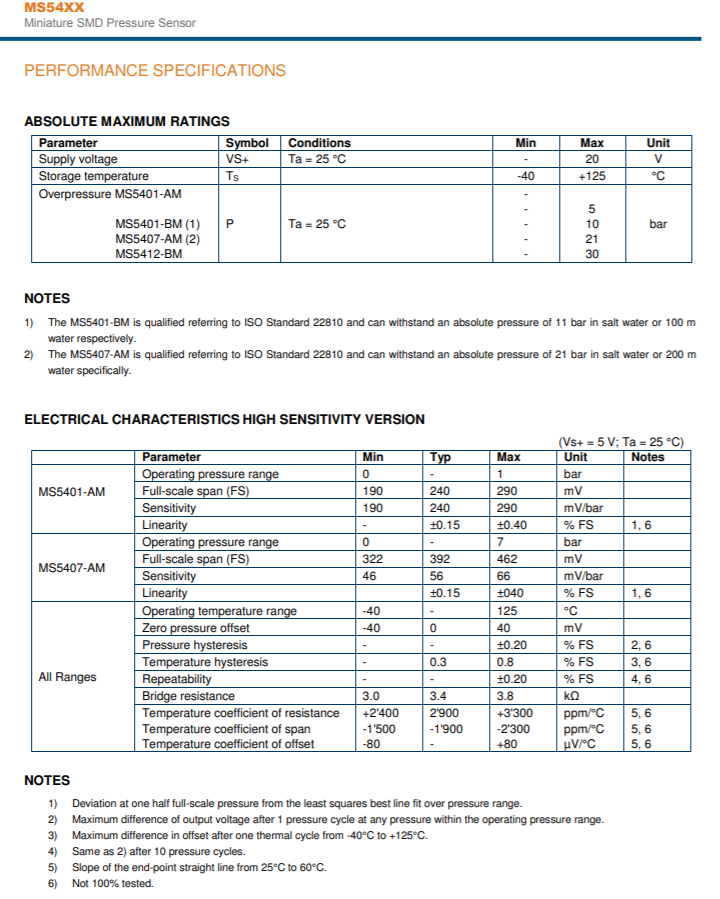
\includegraphics[width=1\columnwidth]{figures/MS5401-AM DS.png}


\end{document}

% DE: things to consider; sensing forces, sensing vibration,
% sensing if flow is attached, sensing lift/drag on fin, 
% sensing "luffing"... we've jumped straight to something about
% vorticity and circulation from an upstream body without
% explaining why; also look up stall sensing for wings, 
% GI taylor vorticity video where he makes little devices 
% track vorticity...